\section{Experimentos}
\label{sec:Experiments}

\paragraph{Detalles de implementación.} Adoptamos SigLiP-so400M\cite{zhai2023siglip} como visual encoder, usamos un MLP como projection head y empleamos Qwen2-7B como LLM. Por defecto, la cantidad de visual tokens está limitada a 8192. Entre ellos, 729 tokens se asignan a percepción en tiempo real, mientras que la memoria espaciotemporal de corto plazo consiste en 18 frames, cada uno representado por 128 visual tokens. Fijamos los pesos de penalización para similitud, conteo de fusiones y distancia temporal en 0.4, 0.4 y 0.2, respectivamente. El modelo se entrena en 32 GPUs A100 usando nuestro dataset propuesto OnlineIT, complementado con datos de video offline de VideoChat-Flash \cite{li2024videochatflash} y LLaVA-Video \cite{zhang2024llavavideo}, así como con datos de imagen de LLaVA-OneVision \cite{li2024llavaov}. Adoptamos una estrategia de entrenamiento de cinco etapas para entrenar StreamForest desde cero. Las primeras tres etapas siguen el paradigma de entrenamiento de MLLMs offline para video largo \cite{li2024videochatflash}. La cuarta etapa realiza fine-tuning de streaming video para obtener StreamForest base. Además, puede incorporarse una quinta etapa opcional entrenando con OnlineIT-Drive, lo que produce StreamForest(FT-drive). Durante la fase de evaluación, restringimos al modelo a procesar frames de streaming a 1 FPS. Para detalles de implementación más específicos, véase el Apéndice \ref{app:sec:More_Implementation_Details}.


\subsection{Resultados en benchmarks online}

Evaluamos el rendimiento de nuestro modelo en cuatro benchmarks de online video question answering: ODV-Bench, StreamingBench \cite{lin2024streamingbench}, OVBench \cite{huang2024videochatonline} y OVO-Bench \cite{li2025ovobench}. Estos benchmarks siguen escenarios de streaming video QA, donde los VideoLLMs deben procesar únicamente el contenido de video disponible antes del timestamp actual.




\begin{table}[t]
\setlength{\tabcolsep}{3pt}
\renewcommand{\arraystretch}{1.3}

    \caption{
        \textbf{Resultados de evaluación en ODV-Bench.} Nuestro modelo supera significativamente a los video MLLMs offline y online de estado del arte bajo condiciones de prueba zero-shot, y logra mejoras adicionales después de fine-tuning con datos del dominio de conducción.
    }

\resizebox{1\textwidth}{!}{%
\begin{tabular}{lcccccccccccccccccc}
\hline \hline
                                       &                                 & \multicolumn{1}{l|}{}                                    & \multicolumn{7}{c|}{\textbf{Static Target}}                                                                                                                                       & \multicolumn{4}{c|}{\textbf{Dynamic Target}}                                                                  & \multicolumn{4}{c|}{\textbf{Event Oriented}}                                                                 &                                    \\ \cline{4-18}
\multirow{-2}{*}{\textbf{Method}}      & \multirow{-2}{*}{\textbf{Size}} & \multicolumn{1}{l|}{\multirow{-2}{*}{\textbf{\#Frames}}} & RTP                  & HD                   & KIE                  & TCD                 & DDM                  & \multicolumn{1}{c|}{PTM} & \multicolumn{1}{c|}{Avg.} & AP                   & LP                   & \multicolumn{1}{c|}{DP}  & \multicolumn{1}{c|}{Avg.} & RP                  & RA                  & \multicolumn{1}{c|}{ARA}  & \multicolumn{1}{c|}{Avg.} & \multirow{-2}{*}{\textbf{Overall}} 
\\ \hline

\multicolumn{19}{l}{\textit{Human}}\\ 
\hline

Human Agents & - & \multicolumn{1}{c|}{-} & 96.8 & 97.6 & 98.2 & 95.7 & 95.9 & \multicolumn{1}{c|}{94.4} & \multicolumn{1}{c|}{95.9} & 83.7 & 87.9 & \multicolumn{1}{c|}{90.4} & \multicolumn{1}{c|}{88.2} & 91.9 & 94.9 & \multicolumn{1}{c|}{93.0} & \multicolumn{1}{c|}{92.5} & 91.4 \\

\hline
\multicolumn{19}{l}{\textit{Open-source Offline Video MLLMs}}\\ 
\hline

MiniCPM-V2.6 \cite{yao2024minicpmv} & 7B & \multicolumn{1}{c|}{64} & 20.0 & \textbf{87.8} & 15.1 & 49.1 & 26.4 & \multicolumn{1}{c|}{20.6} & \multicolumn{1}{c|}{27.3} & 71.2 & 73.4 & \multicolumn{1}{c|}{47.2} & \multicolumn{1}{c|}{60.0} & \textbf{73.4} & 33.3 & \multicolumn{1}{c|}{16.7} & \multicolumn{1}{c|}{53.6} & 49.8 \\

LongVA \cite{zhang2024longva} & 7B & \multicolumn{1}{c|}{64} & 29.9 & 7.3 & 37.7 & 47.3 & \textbf{38.0} & \multicolumn{1}{c|}{33.6} & \multicolumn{1}{c|}{31.8} & 66.6 & 58.6 & \multicolumn{1}{c|}{\textbf{50.9}} & \multicolumn{1}{c|}{56.6} & 57.5 & 58.1 & \multicolumn{1}{c|}{46.2} & \multicolumn{1}{c|}{56.7} & 50.2 \\

LLaVA-Onevision \cite{li2024llavaov} & 7B & \multicolumn{1}{c|}{64} & 36.0 & 4.9 & 22.6 & 60.0 & 31.4 & \multicolumn{1}{c|}{39.0} & \multicolumn{1}{c|}{34.2} & 53.6 & 70.3 & \multicolumn{1}{c|}{47.4} & \multicolumn{1}{c|}{55.1} & 57.9 & 72.2 & \multicolumn{1}{c|}{47.4} & \multicolumn{1}{c|}{62.2} & 51.6 \\

InternVL2.5 \cite{chen2024internvl2_5} & 8B & \multicolumn{1}{c|}{32} & 40.1 & 16.3 & 37.7 & 52.7 & 30.4 & \multicolumn{1}{c|}{40.9} & \multicolumn{1}{c|}{37.2} & 64.1 & \textbf{84.6} & \multicolumn{1}{c|}{49.5} & \multicolumn{1}{c|}{\textbf{62.5}} & 54.0 & 60.6 & \multicolumn{1}{c|}{50.6} & \multicolumn{1}{c|}{56.1} & 54.2 \\

VideoChat-Flash \cite{li2024videochatflash} & 7B & \multicolumn{1}{c|}{256} & 29.6 & 15.5 & 45.3 & \textbf{76.4} & 26.1 & \multicolumn{1}{c|}{36.1} & \multicolumn{1}{c|}{32.2} & \textbf{73.5} & 75.3 & \multicolumn{1}{c|}{47.2} & \multicolumn{1}{c|}{61.0} & 67.1 & 64.8 & \multicolumn{1}{c|}{46.2} & \multicolumn{1}{c|}{\textbf{64.3}} & 54.4 \\

Qwen2.5-VL \cite{bai2025qwen2_5vl} & 7B & \multicolumn{1}{c|}{1fps} & \textbf{51.8} & 8.1 & \textbf{79.3} & 49.1 & 36.0 & \multicolumn{1}{c|}{\textbf{57.3}} & \multicolumn{1}{c|}{\textbf{48.3}} & 50.4 & 82.6 & \multicolumn{1}{c|}{46.9} & \multicolumn{1}{c|}{57.5} & 47.6 & \textbf{78.6} & \multicolumn{1}{c|}{\textbf{52.6}} & \multicolumn{1}{c|}{59.4} & \textbf{55.6} \\ 


\hline
\multicolumn{19}{l}{\textit{Open-source Online Video MLLMs}}\\ 
\hline


Flash-VStream \cite{zhang2024flashvstream} & 7B & \multicolumn{1}{c|}{1fps} & 25.4 & 1.6 & 11.3 & 50.9 & 36.0 & \multicolumn{1}{c|}{22.1} & \multicolumn{1}{c|}{24.8} & 25.5 & 39.8 & \multicolumn{1}{c|}{47.2} & \multicolumn{1}{c|}{40.2} & 32.4 & 48.6 & \multicolumn{1}{c|}{30.1} & \multicolumn{1}{c|}{38.1} & 35.7 \\

Dispider \cite{qian2025dispider} & 7B & \multicolumn{1}{c|}{1fps} & 31.1 & 7.3 & 34.0 & 63.6 & 34.0 & \multicolumn{1}{c|}{35.4} & \multicolumn{1}{c|}{32.5} & 43.2 & 73.1 & \multicolumn{1}{c|}{45.8} & \multicolumn{1}{c|}{52.7} & 38.2 & 55.4 & \multicolumn{1}{c|}{36.5} & \multicolumn{1}{c|}{44.3} & 45.2 \\

VideoChat-Online \cite{huang2024videochatonline} & 4B & \multicolumn{1}{c|}{1fps} & 36.9 & 0.8 & 62.3 & 49.1 & 21.5 & \multicolumn{1}{c|}{47.0} & \multicolumn{1}{c|}{36.1} & 70.2 & 86.7 & \multicolumn{1}{c|}{46.4} & \multicolumn{1}{c|}{62.9} & 51.2 & 69.4 & \multicolumn{1}{c|}{45.5} & \multicolumn{1}{c|}{57.4} & 54.5 \\ 

\rowcolor[HTML]{DFF7DC}
\textbf{StreamForest} & \textbf{7B} & \multicolumn{1}{c|}{\textbf{1fps}} & 51.4 & 15.5 & 54.7 & 56.4 & \textbf{38.6} & \multicolumn{1}{c|}{65.3} & \multicolumn{1}{c|}{51.5} & \textbf{72.6} & 83.2 & \multicolumn{1}{c|}{46.0} & \multicolumn{1}{c|}{62.3} & 60.2 & 73.3 & \multicolumn{1}{c|}{47.4} & \multicolumn{1}{c|}{63.8} & {59.9} \\

\rowcolor[HTML]{DFF7DC}
\textbf{StreamForest (FT-drive)} & \textbf{7B} & \multicolumn{1}{c|}{\textbf{1fps}} & \textbf{70.1} & \textbf{17.1} & \textbf{100.0} & \textbf{60.0} & 32.7 & \multicolumn{1}{c|}{\textbf{83.6}} & \multicolumn{1}{c|}{\textbf{64.6}} & 64.0 & \textbf{96.6} & \multicolumn{1}{c|}{\textbf{59.6}} & \multicolumn{1}{c|}{\textbf{70.7}} & \textbf{71.8} & \textbf{93.4} & \multicolumn{1}{c|}{\textbf{58.3}} & \multicolumn{1}{c|}{\textbf{78.5}} & \textbf{71.2} \\ 

\hline \hline

\end{tabular}%
}

    % \vspace{-10pt}
    \label{tab:Benchmark_Ours}
\end{table}


\paragraph{ODV-Bench.} Integra estrechamente información espaciotemporal para evaluar de forma integral la capacidad de los MLLMs para comprender detalles finos en videos online y realizar predicciones futuras basadas tanto en contexto histórico como actual en escenarios de conducción autónoma. El benchmark incluye tareas como identificar objetos o acciones sutiles, describir posiciones de objetos y relaciones espaciales, y predecir trayectorias de objetos. Estas tareas requieren una sólida percepción espaciotemporal en tiempo real y comprensión contextual. Como se muestra en la Tabla \ref{tab:Benchmark_Ours}, StreamForest alcanza una exactitud promedio de 59.9\% en ODV-Bench sin ser entrenado con OnlineIT-drive y mejora aún más hasta 71.2\% después de entrenarse con él. Esto supera significativamente a todos los MLLMs online y offline existentes, demostrando la fuerte capacidad de generalización de nuestro método hacia tareas downstream de streaming video understanding. Estos resultados resaltan su potencial para aplicaciones del mundo real.





\begin{table}[t]
    \centering
    \renewcommand{\arraystretch}{1.2}
    \setlength{\tabcolsep}{6pt}


    \caption{
        \textbf{Comparación de nuestro método con enfoques existentes en tareas de video question answering bajo diversos escenarios.} Nuestro enfoque supera significativamente a los métodos previos en benchmarks de comprensión de streaming video, al tiempo que mantiene un rendimiento sólido y competitivo tanto en comprensión de video largo como corto.
    }

    
    \resizebox{1\textwidth}{!}{
        \begin{tabular}{lcccccccc}
            \hline \hline
            \multirow{3}{*}{\textbf{Method}} & \multicolumn{1}{c|}{\multirow{3}{*}{\textbf{Size}}} & \multicolumn{3}{c|}{\textbf{Online Video}} & \multicolumn{2}{c|}{\textbf{Long Video}} & \multicolumn{2}{c}{\textbf{Short Video}} \\ \cline{3-9} 
             & \multicolumn{1}{c|}{} & \textbf{StreamingBench} & \textbf{OVBench} & \multicolumn{1}{c|}{\textbf{OVO-Bench}} & \textbf{VideoMME} & \multicolumn{1}{c|}{\textbf{MLVU}} & \textbf{MVBench} & \textbf{PerceptionTest} \\
             & \multicolumn{1}{c|}{} & Real-Time All & Avg & \multicolumn{1}{c|}{Overall} & w/o sub. & \multicolumn{1}{c|}{M-Avg} & Avg & Val \\ \hline

            \multicolumn{9}{l}{\textit{Open-source Offline Video MLLMs}} \\ 
            \hline
            
            InternVL2 \cite{chen2024internvl2} & \multicolumn{1}{c|}{8B} & 63.7 & 48.7 & \multicolumn{1}{c|}{50.1} & 54.0 & \multicolumn{1}{c|}{64.0} & 65.8 & - \\
            
            LongVA \cite{zhang2024longva} & \multicolumn{1}{c|}{7B} & 60.0 & 43.6 & \multicolumn{1}{c|}{-} & 52.6 & \multicolumn{1}{c|}{56.3} & - & - \\
            
            LLaVA-OneVision \cite{li2024llavaov} & \multicolumn{1}{c|}{7B} & 71.1 & 49.5 & \multicolumn{1}{c|}{52.9} & 58.2 & \multicolumn{1}{c|}{64.7} & 56.7 & 57.1 \\
            
            Qwen2-VL \cite{qwen2vl} & \multicolumn{1}{c|}{7B} & 69.0 & 49.7 & \multicolumn{1}{c|}{52.7} & 63.3 & \multicolumn{1}{c|}{-} & 67.0 & 66.9 \\
            
            LongVU \cite{shen2024longvu} & \multicolumn{1}{c|}{7B} & - & - & \multicolumn{1}{c|}{48.5} & 60.6 & \multicolumn{1}{c|}{65.4} & 66.9 & - \\
            
            LLaVA-Video \cite{zhang2024llavavideo} & \multicolumn{1}{c|}{7B} & - & - & \multicolumn{1}{c|}{53.1} & 63.3 & \multicolumn{1}{c|}{70.8} & 58.6 & 67.9 \\ \hline
            
            \multicolumn{9}{l}{\textit{Open-source Online Video MLLMs}} \\ \hline
            
            VideoLLM-online \cite{chen2024videollmonline} & \multicolumn{1}{c|}{8B} & 36.0 & 9.6 & \multicolumn{1}{c|}{12.8} & - & \multicolumn{1}{c|}{-} & - & - \\
            
            MovieChat \cite{song2024moviechat} & \multicolumn{1}{c|}{7B} & - & 30.9 & \multicolumn{1}{c|}{-} & 38.2 & \multicolumn{1}{c|}{-} & 55.1 & - \\
            
            Flash-VStream \cite{zhang2024flashvstream} & \multicolumn{1}{c|}{7B} & 23.2 & 31.2 & \multicolumn{1}{c|}{33.2} & - & \multicolumn{1}{c|}{-} & - & - \\
            
            VideoChat-Online \cite{huang2024videochatonline} & \multicolumn{1}{c|}{4B} & - & 54.9 & \multicolumn{1}{c|}{-} & 52.8 & \multicolumn{1}{c|}{-} & 64.9 & - \\
            
            Dispider \cite{qian2025dispider} & \multicolumn{1}{c|}{7B} & 67.6 & - & \multicolumn{1}{c|}{41.8} & 57.2 & \multicolumn{1}{c|}{61.7} & - & - \\ 

            \rowcolor[HTML]{DFF7DC}
            \textbf{StreamForest} & \multicolumn{1}{c|}{\textbf{7B}} & \textbf{77.3} & \textbf{60.5} & \multicolumn{1}{c|}{\textbf{55.6}} & \textbf{61.4} & \multicolumn{1}{c|}{\textbf{70.0}} & \textbf{70.2} & \textbf{73.1} \\ 
            
            \rowcolor[HTML]{DFF7DC}
            \textbf{StreamForest (FT-drive)} & \multicolumn{1}{c|}{\textbf{7B}} & \textbf{76.8} & \textbf{61.6} & \multicolumn{1}{c|}{\textbf{55.6}} & \textbf{61.9} & \multicolumn{1}{c|}{\textbf{69.6}} & \textbf{68.6} & \textbf{71.6} \\ 
            
            \hline \hline
            
        \end{tabular}
    }
    

    
    \label{tab:Benchmark_Others}
    % \vspace{-10pt}
\end{table}



\paragraph{StreamingBench \& OVBench \& OVO-Bench.} Como se muestra en la Tabla \ref{tab:Benchmark_Others}, StreamForest demuestra un rendimiento sólido en los benchmarks open-source existentes de streaming video understanding. Alcanza una exactitud de 77.3\% en StreamingBench, 60.5\% en OVBench y 55.6\% en OVO-Bench. Estos resultados destacados subrayan la robustez de StreamForest en una amplia gama de escenarios de online video understanding. El rendimiento superior de nuestro modelo puede atribuirse a dos innovaciones arquitectónicas clave. Primero, la Fine-grained Spatiotemporal Window permite percepción espacial precisa y modelado temporal reactivo de corto plazo, ambos críticos para tareas de percepción en tiempo real y respuesta hacia adelante. Segundo, el Persistent Event Memory Forest organiza adaptativamente contenido visual de largo plazo en un bosque de memoria estructurado y eficiente, mejorando significativamente la capacidad del MLLM para retener y razonar sobre eventos pasados. En conjunto, estos dos módulos ofrecen capacidades complementarias que permiten a nuestro modelo manejar eficazmente entradas dinámicas de streaming video de largo horizonte, manteniendo al mismo tiempo alta coherencia contextual.



\subsection{Resultados en benchmarks offline}



Además evaluamos nuestro método en dos benchmarks de long video understanding (VideoMME\cite{fu2024videomme} y MLVU\cite{zhou2024mlvu}) y dos datasets de video corto (MVBench\cite{li2024mvbench} y PerceptionTest\cite{patraucean2023perceptiontest}). En el escenario offline, el video completo se proporciona como entrada al MLLM. Muestreamos frames de video a 1 FPS, con un límite máximo de 2048 frames. Para los videos que exceden este límite, los frames se muestrean uniformemente a lo largo de toda la duración. Como se muestra en la Tabla \ref{tab:Benchmark_Others}, nuestro método demuestra un rendimiento superior tanto en tareas de video understanding largo como corto en comparación con los recientes online Video MLLMs de estado del arte. Además, supera a modelos offline líderes en la mayoría de los benchmarks, logrando 61.4\% en VideoMME, 70.0\% en MLVU, 70.2\% en MVBench y 73.1\% en PerceptionTest. Este sólido rendimiento en escenarios offline resalta la robusta capacidad de generalización de nuestro método propuesto.

\subsection{Ablaciones}

\paragraph{Efectividad de Persistent Event Memory Forest:}
Reemplazamos el PEMF propuesto por varios métodos usados en trabajos previos. Para asegurar una comparación justa, mantenemos consistentes los presupuestos de visual tokens en todos los métodos y realizamos fine-tuning de cada modelo en consecuencia. Los resultados de ablación se muestran en la Tabla \ref{tab:ablation_PEMF}. La estrategia FIFO muestra el peor rendimiento. Esto es especialmente evidente en el benchmark de video largo MLVU (56.7\% vs. 70.0\%), donde el método falla debido al descarte sin filtrado de características visuales históricas. OVBench enfatiza principalmente percepción espaciotemporal fina y de corto plazo. El muestreo uniforme reduce la resolución de la información visual reciente, que es crucial para la comprensión en tiempo real (58.2\% vs. 60.5\% en OVBench). Similarity Merge logra un rendimiento comparable al de nuestro PEMF en OVBench (60.3\% vs. 60.5\%). Sin embargo, sus limitaciones se vuelven claras en tareas que requieren memoria persistente y razonamiento de largo horizonte. En OVO-Bench, PEMF supera a Similarity Merge en +2.2\%, y en MLVU en +2.0\%. Esto se debe a que la fusión basada en similitud puede fusionar en exceso frames dentro de segmentos locales de video, lo que podría conducir a irregularidades espaciotemporales y a la pérdida de representaciones locales a nivel de evento. El pyramidal memory bank mantiene memoria mediante reemplazo de frames. Sin embargo, la capacidad fija limita su habilidad para capturar características espaciotemporales de largo alcance (53.9\% vs. 55.6\% en OVO-Bench y 68.2\% vs. 70.0 en MLVU). En contraste, nuestro método evalúa cada evento visual según similitud a nivel de evento, conteo de fusiones y distancia temporal. Luego realiza consolidación de memoria a nivel de evento. Esta estrategia soporta un mantenimiento eficiente y persistente de características visuales históricas.




\paragraph{Efectividad de la arquitectura completa:}
Realizamos estudios de ablación sobre tres componentes arquitectónicos clave. En particular, ablatimos la Fine-grained Spatiotemporal Window y el Persistent Event Memory Forest, garantizando al mismo tiempo que el número total de visual tokens se mantenga consistente con la configuración original. Además, reemplazamos la construcción de nodos basada en eventos por un enfoque basado en frames. Como se muestra en la Tabla \ref{tab:ablation_structure}, eliminar ambos módulos conduce a la caída de rendimiento más significativa. Usar solo FSTW o solo PEMF mejora el rendimiento en comparación con el baseline, pero los mejores resultados se logran cuando ambos componentes se integran (+2.5\% en OVBench, +3.1\% en OVO-Bench y +18.2\% en MLVU). Esta ablación conjunta confirma que FSTW y PEMF proporcionan beneficios complementarios. FSTW mejora la percepción espaciotemporal en tiempo real cerca del timestamp de la consulta, mientras que PEMF soporta una memoria de largo plazo eficiente y persistente, produciendo juntos el rendimiento global más fuerte. Además, la construcción de nodos a nivel de evento previene eficazmente la sobre-fusión dentro de los eventos, permitiendo comprimir características visuales al nivel de eventos visuales completos en lugar de frames individuales.

% Please add the following required packages to your document preamble:
% \usepackage{multirow}
\begin{table}[t]
    \begin{minipage}[t]{0.52\linewidth}
        % \vspace{0pt}
        \centering
        \setlength{\tabcolsep}{3pt}
        \renewcommand{\arraystretch}{1.1}

        \caption{
            Comparación entre nuestro PEMF propuesto y otras estrategias de memoria de uso común.
        }
        
        \resizebox{1\textwidth}{!}{
            \begin{tabular}{l|ccc}
            \hline
             & \textbf{OVBench} & \textbf{OVO-Bench} & \textbf{MLVU}  \\
            \multirow{-2}{*}{\textbf{Memory Policy}} & Avg & Overall & M-Avg  \\ \hline
            Uniform Sampling & 58.2 & 52.7 & 69.4  \\
            First In First Out & 58.7 & 52.9 & 56.7  \\
            Similarity Merge \cite{song2024moviechat} & 60.3 & 53.4 & 68.0  \\
            Pyramid Memory Bank \cite{huang2024videochatonline} & 60.3 & 53.9 & 68.2  \\
            \rowcolor[HTML]{DFF7DC}
            \textbf{PEMF (Ours)} & \textbf{60.5} & \textbf{55.6} & \textbf{70.0}  \\ \hline
            \end{tabular}
        }
        % \vspace{5pt}

        \label{tab:ablation_PEMF}
    \end{minipage}
    \hspace{2pt}
    \begin{minipage}[t]{0.46\linewidth}
        % \vspace{0pt}
        \centering
        \setlength{\tabcolsep}{3pt}
        \renewcommand{\arraystretch}{1.1}

        \caption{
            Estudio de ablación sobre los componentes clave de StreamForest.
        }
        
        \resizebox{1\textwidth}{!}{
            \begin{tabular}{l|ccc}
            \hline
             & \textbf{OVBench} & \textbf{OVO-Bench} & \textbf{MLVU}  \\
            \multirow{-2}{*}{\textbf{Model}} & Avg & Overall & M-Avg  \\ \hline
            w/o FSTW \& PEMF & 58.0 & 52.5 & 51.8  \\
            w/o FSTW & 59.1 & 53.7 & 69.4  \\
            w/o PEMF & 58.9 & 53.5 & 56.6  \\
            w/o Event & 59.4 & 52.6 & 69.1  \\
            \rowcolor[HTML]{DFF7DC} 
            \textbf{Ours} & \textbf{60.5} & \textbf{55.6} & \textbf{70.0}  \\ \hline
            \end{tabular}
        }
        % \vspace{5pt}

        \label{tab:ablation_structure}
    \end{minipage}

% \vspace{-0.4cm}
    
\end{table}

\begin{figure}[h]
    \centering
    \begin{minipage}[t]{0.48\textwidth}
        \centering
        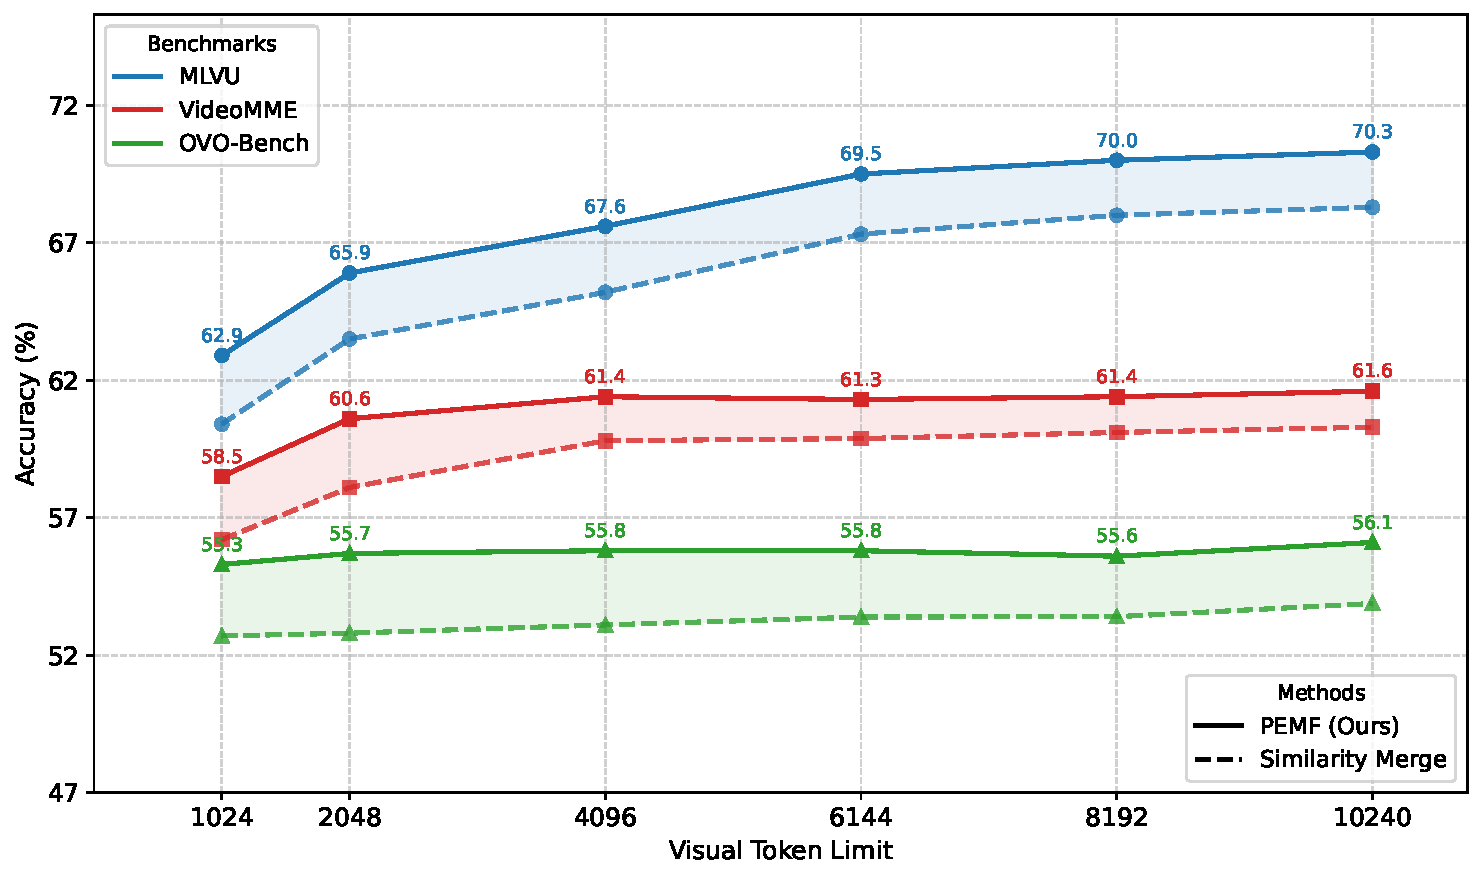
\includegraphics[width=\linewidth]{figs/ablation_length_img.pdf}
        \caption{
            Rendimiento bajo distintos presupuestos de visual tokens.
        }
        \label{fig:token_budget}
    \end{minipage}%
    \hfill
    \begin{minipage}[t]{0.48\textwidth}
        \centering
        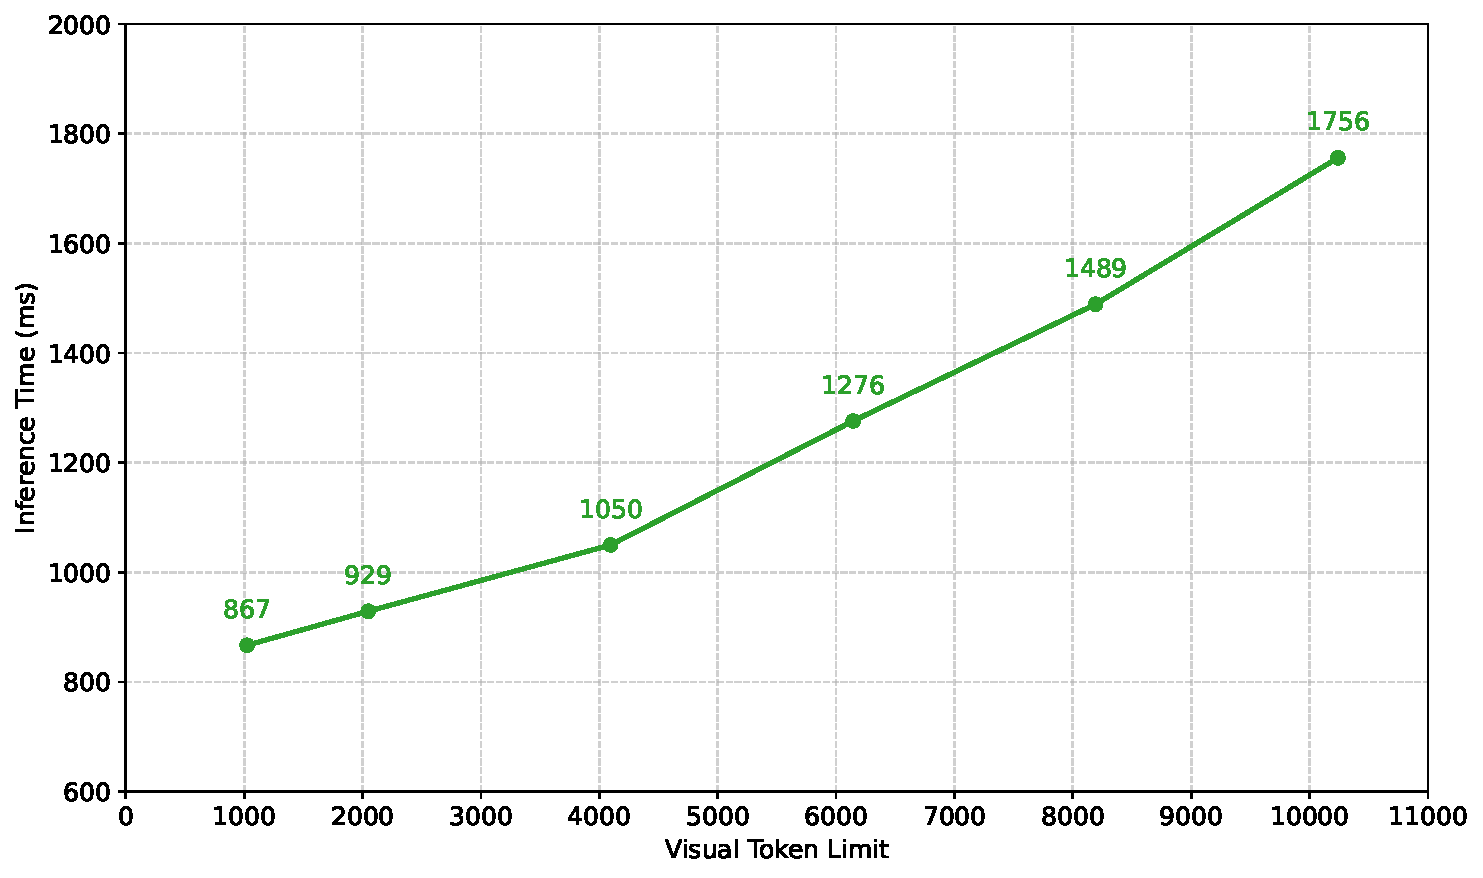
\includegraphics[width=\linewidth]{figs/ablation_inference_time.pdf}
        \caption{
            Tiempo promedio de inferencia bajo distintos presupuestos de visual tokens (en una sola GPU A100).
        }
        \label{fig:token_budget_time}
    \end{minipage}%
    
\end{figure}




\paragraph{Robustez ante distintos presupuestos de visual tokens:}
Evaluamos la robustez de nuestro método bajo distintas restricciones presupuestarias para visual tokens, desde 1K hasta 10K. La Figura \ref{fig:token_budget} ilustra la variación del rendimiento en los benchmarks MLVU, VideoMME y OVO-Bench bajo estas configuraciones. Notablemente, bajo la restricción estricta de solo 1K visual tokens, StreamForest alcanza una tasa promedio de compresión visual de hasta 99.8\% en benchmarks de video largo. A pesar de este nivel extremo de compresión, el modelo aún mantiene un rendimiento competitivo, lo que demuestra con fuerza la robustez de nuestro enfoque para preservar persistentemente memorias visuales de largo plazo a nivel de evento.
%
También realizamos una comparación directa entre nuestro PEMF y Similarity Merge. Los resultados demuestran claramente dos beneficios centrales de nuestro enfoque. Primero, PEMF exhibe un rendimiento absoluto superior, superando consistentemente a Similarity Merge en todos los presupuestos de tokens con una mejora promedio de exactitud de 2--3\%. Segundo, nuestro método muestra mayor resiliencia frente a compresión extrema. Bajo el presupuesto más severo de 1K tokens, PEMF retiene una fracción más alta de su rendimiento con presupuesto completo, logrando una ventaja relativa notable de retención de +1.8\% en VideoMME. Estos resultados experimentales confirman que las ganancias de rendimiento provienen del diseño intrínseco de PEMF, que consolida adaptativamente memoria a nivel de evento para preservar información semánticamente saliente, asegurando así tanto alta exactitud como eficiencia de tokens bajo restricciones estrictas de recursos.
%
La Figura \ref{fig:token_budget_time} presenta el tiempo promedio de inferencia de StreamForest bajo distintos presupuestos de visual tokens. La velocidad de inferencia rápida y estable resalta la aplicabilidad práctica de StreamForest.


% Please add the following required packages to your document preamble:
% \usepackage{multirow}
% \usepackage{colortbl}
% \usepackage{graphicx}
\begin{table}[t]
    \begin{minipage}[t]{0.40\linewidth}
        \centering
        \setlength{\tabcolsep}{4pt}
        \renewcommand{\arraystretch}{1.1}

        \caption{
            Análisis cuantitativo del tiempo de ejecución y el uso de memoria de StreamForest. 
        }
        
        \resizebox{1\textwidth}{!}{
            \begin{tabular}{c|c|c|c}
            \hline
            \textbf{Input Frames} & \textbf{Memory (GB)} & \textbf{FLOPs (T)} & \textbf{Latency (s)} \\ \hline
            64   & 15.8 & 93.1  & 0.776 \\
            256  & 17.1 & 134.1 & 1.126 \\
            1024 & 17.2 & 137.3 & 1.497 \\ \hline
            \end{tabular}
        }

        \label{tab:runtime_memory}
    \end{minipage}
    \hspace{3pt}
    \begin{minipage}[t]{0.58\linewidth}
        \centering
        \setlength{\tabcolsep}{4pt}
        \renewcommand{\arraystretch}{1.1}

        \caption{
            Comparación del tiempo de ejecución de PEMF con otros mecanismos de memoria para 500 frames. 
        }
        
        \resizebox{1\textwidth}{!}{
            \begin{tabular}{l|c|c|c|c}
            \hline
            \textbf{Method} & \textbf{Vis. Encode (s)} & \textbf{Mem. Update (s)} & \textbf{LLM infer (s)} & \textbf{Total (s)} \\ \hline
            Similarity Merge \cite{song2024moviechat} & 5.198 & 0.183 & 1.388 & 6.769 \\
            PMB \cite{huang2024videochatonline} & 5.203 & 0.451 & 1.381 & 7.035 \\
            \rowcolor[HTML]{DFF7DC}
            \textbf{PEMF (Ours)} & 5.218 & \textbf{0.172} & 1.394 & 6.784 \\ \hline
            \end{tabular}
        }

        \label{tab:memory_mechanism_comparison}
    \end{minipage}
\end{table}



\paragraph{Costo computacional:} 
Proporcionamos un análisis cuantitativo del tiempo de ejecución y el uso de memoria de StreamForest. Para aislar el efecto del mecanismo de memoria, asumimos que las características visuales a nivel de frame ya han sido extraídas por el vision encoder en tiempo real. Como se muestra en la Tabla \ref{tab:runtime_memory}, PEMF impone un límite superior estricto de visual tokens (8K aquí), garantizando que el uso de memoria permanezca estable (\~17 GB) independientemente del número de frames procesados. En consecuencia, los FLOPs y la latencia de inferencia no crecen significativamente incluso con entradas de streaming más largas.
%
Además, comparamos PEMF con otros mecanismos de memoria, incluyendo Pyramid Memory Bank \cite{huang2024videochatonline} y la estrategia Similarity Merge \cite{song2024moviechat}. Como se resume en la Tabla \ref{tab:memory_mechanism_comparison}, el tiempo total de ejecución está dominado por el vision encoding (5.2s para 500 frames, $\sim$95 FPS). La actualización de memoria de PEMF es extremadamente ligera (0.172s para 500 frames), lo cual es despreciable en comparación con las ganancias de eficiencia obtenidas al reducir significativamente la cantidad total de visual tokens. 
% The experiments in the Appendix \ref{app:sec:Efficiency_Multi-round} also demonstrate the high computational efficiency of StreamForest in multi-turn conversational scenarios.


\begin{wraptable}{r}{0.40\textwidth}
    \vspace{-10pt}
    \centering
    \renewcommand{\arraystretch}{1.2}
    \setlength{\tabcolsep}{2pt}
    \caption{
        La contribución de nuestros datos de entrenamiento al rendimiento en el benchmark de streaming video understanding. O.general se refiere a OnlineIT-general, mientras que O.drive se refiere a OnlineIT-drive.
    }
    
    \resizebox{0.40\textwidth}{!}{
        \begin{tabular}{l|ccc}
        \hline
        \multirow{2}{*}{\textbf{Data}} & \textbf{ODV-Bench} & \textbf{OVBench} & \textbf{OVO-Bench} \\
         & Avg & Avg & Overall \\ \hline
        base & 56.3 & 53.9 & 53.5 \\
        \rowcolor[HTML]{DFF7DC} base + O.general & 59.9 & 60.5 & \textbf{55.6} \\
        \rowcolor[HTML]{DFF7DC} base + O.general + O.drive & \textbf{71.2} & \textbf{61.6} & \textbf{55.6} \\ \hline
        \end{tabular}
    }
    \label{tab:ablation_dataset}
    % \vspace{-10pt}
\end{wraptable}

\paragraph{Impacto de los datos de entrenamiento:}
La Tabla \ref{tab:ablation_dataset} presenta el impacto de nuestra estrategia de entrenamiento que integra tanto datasets online como offline. Los resultados demuestran claramente que combinar OnlineIT con datasets existentes de offline VideoQA mejora significativamente el rendimiento en benchmarks de streaming video understanding. OnlineIT está diseñado específicamente para percepción en tiempo real y predicción futura en escenarios de streaming, mitigando eficazmente las alucinaciones causadas por inconsistencias entre el contexto espaciotemporal histórico y el momento actual.






